\documentclass[journal]{IEEEtran}
\usepackage{tikz}
\usepackage{cite}
\usetikzlibrary{decorations.pathreplacing,angles,quotes}

% correct bad hyphenation here
\hyphenation{op-tical net-works semi-conduc-tor}

\begin{document}
%
% paper title
\title{Project Report}

% puts info about authors at bottom of first page
\author{Lawrence~Owusu,~Jordan~Sturtz,~and~Swetha~Chittam~% <-this % stops a space
  \thanks{The authors are graduate students at NCA\&T}% <-this % stops a space
}

% note the % following the last \IEEEmembership and also \thanks -
% these prevent an unwanted space from occurring between the last author name
% and the end of the author line. i.e., if you had this:
% \author{....lastname \thanks{...} \thanks{...} }
%                     ^------------^------------^----Do not want these spaces!

% The paper headers
% The only time the second header will appear is for the odd numbered pages
% after the title page when using the twoside option.
\markboth{CS851 - Deep Learning: Project Report}%
{Shell \MakeLowercase{\textit{et al.}}: CS851 - Deep Learning: Project Report}

% make the title area
\maketitle

% As a general rule, do not put math, special symbols or citations
% in the abstract or keywords.
\begin{abstract}
Abstract - clearly state problem, method, and results.
\end{abstract}

% Note that keywords are not normally used for peerreview papers.
% \begin{IEEEkeywords}
% IEEE, IEEEtran, journal, \LaTeX, paper, template.
% \end{IEEEkeywords}

% For peer review papers, you can put extra information on the cover
% page as needed:
% \ifCLASSOPTIONpeerreview
% \begin{center} \bfseries EDICS Category: 3-BBND \end{center}
% \fi

%
% For peerreview papers, this IEEEtran command inserts a page break and
% creates the second title. It will be ignored for other modes.
\IEEEpeerreviewmaketitle

\section{Introduction}
  \IEEEPARstart{P}{rotein} structure sequencing remains one of the challenges in the field of computational biology.
    Determination of accurate protein structure is important in developing deep understanding of the
    functions of proteins and their applications of drug and inhibitor discovery and design.

    Protein sequencing begins in the lab using techniques such as mass spectrometry or Edman degradation
    to identify partial sequences of proteins \cite{mann2016rise, edman1949method}. Various techniques exist for using these
    partial sequences to construct the full protein sequence
    \cite{standing2003peptide,perkins1999probability, eng1994approach, yang2021full}.

    In our paper, we develop an approach using deep learning techniques to predict missing gaps in peptide sequences.
    Our approach begins with a partial sequence with gaps of known size. To retrieve the relevant training data,
    we query the National Center For Biotechnology Information (NCBI) Protein Blast server to retrieve the highest matching
    homologous sequences to our partial sequence \cite{ncbi}. We train two models: one to predict peptides in the forward direction and one to predict in the reverse direction.
    We then use both predictions to predict the missing peptides. Our deep learning models use LSTM layers to learn the
    forward and reverse dependencies.

    \subsection{Related Work}
    % Related work should incldue current progress in sequencing, Genome sequencing and single cell sequencing.
    % Should also refer to paper we are using as our basis for our project.
    % Use google scholar to find those who cited our paper and those citations the paper has.

    The history of using Mass Spectrometry to sequence proteins dates to several years ago.
    In this approach, multiple proteases are employed to cleave the same protein sample separately.
    Because the cleavage of protein by the protease generates overlapping peptides, merging the spectral
    pairs of the overlapping peptides consecutively assembles into long contigs from which de novo
    sequences are obtained \cite{liu2014novo}.

    Some researchers on protein sequencing problems focus on identifying proteins or generating full protein sequences
    by comparing partial sequences to known protein databases to infer the missing gaps in mass spectral data
    \cite{eng1994approach, perkins1999probability}. Others focus on developing techniques for de novo protein sequencing,
    which refers to the process of sequencing proteins without the use of a protein database or with minimal use of
    genomic data \cite{standing2003peptide, bandeira2008automated}.

    Over the last 10 years, de novo protein sequencing has been researched
    extensively in computational proteomics and have been used successfully to deduce peptide sequence
    of un-sequenced organisms, antibodies and post-translastionally modified peptides
    \cite{ma2012novo,veltman2012novo, bandeira2007spectral}. For example,
    Mai et al. reported that their assembling algorithm, Multiple Contigs and Scaffolding
    successfully assembles the de novo identified peptides in contig-scaffold fashion, resulting in
    100\% coverage and 98.69-100\% accuracy on three proteins and replications. The Multiple Contigs
    and Scaffolding algorithm has provided robust and accurate software for full-length protein sequencing
    after de novo identification of peptides \cite{mai2022highly}

    Similarly, Yang et al. reported 100\% accuracy for full-length de novo sequencing
    for light chains of Herceptin and bovine serum albumin (BSA) when their proposed method was applied to de novo
    sequencing of bovine serum albumin (BSA) and monoclonal antibody Herceptin. However, the accuracy marginally dropped to
    99.7\% for the heavy chains of Herceptin \cite{yang2021full}.

    Protein sequencing is only one type of sequencing problem in biology. Related types of sequencing problems include
    single-cell protein sequencing or whole genomic sequencing \cite{wang2015advances,pareek2011sequencing}.

\section{Method}

%   Method: Should have two subsctions (1) Data discussion (preprocessing, where we got it from etc), (2) LSTM / CNN model
  \subsection{Data Collection}
    For our initial project, we used as a target sequence the light chain of alemtuzumab referenced in Liu, et al.
    \cite{liu2014novo}. We manually removed the gaps produced by Liu et al.'s tandem mass spectrometry approach, then
    entered that sequence into NCBI's Protein Blast Server to retrieve the closest matching homologous sequences \cite{ncbi}.
    We used the top ten homologous sequences as training data. The closest matching homologous sequences in our training
    data range from 89.32\% to 82.52\% similarity.

  \subsection{Data Preprocessing}
  We generated from our homologous sequences all kmers. A Kmer is a any substring of length K. For our models, we chose a
  kmer-length of 5. Each kmer represents a single input. The output of each associated kmer is the next character in the sequence.
  Thus, for instance, if one of our homologous sequences contains the substring "DIQM", then a single training instance would be
  the input-output tuple (DIQ, M).

  From our ten homologous sequences, we generated 2106 number of input-output pairs with an input length of 5.
  The kmer length will represent the timesteps in our LSTM layer.
  To be fed into a neural network, the data must be encoded numerically, so we assigned integer labels to each character.
  The output of each training instance is a
  one-hot encoded vector to represent the target classes. Since we are training two models, one for forward prediction
  and one for reverse prediction, we generate the same training data in both the reverse and forward directions.

  The samples of forward and reverse input-output pairs are divided into train and validation sets with the ratio of
  90\% and 10\% respectively. The validation set is used to perform hyperparameter tuning.

\subsection{Data Normalization}
    The input pairs are normalized by dividing with number of classes to obtain a range between [0, 1].
    The number of classes are determined by extracting all the unique characters from the input sequences.
    This data normalization technique is applied to forward, reverse and test data input-output pairs.
    Normalization helps speed the training process.

  \subsection{Model Overview}

    For our sequence prediction task, we built four deep learning models combining convolutional neural
    networks (CNN) with long short term memory (LSTM). The CNN layer helps with automatic feature extraction, in particular
    if there are patterns within each kmer that can be extracted for better predictions. The LSTM layer learns
    the dependencies in the sequence data to predict the correct output. For our four hybrid models, we also
    added two dense hidden layers with ReLu activation and a final output layer with softmax activation.

    Our four hybrid models are LSTM, CNN-LSTM, Bi-LSTM, and CNN-Bi-LSTM.
    The purpose of using four models is to compare their results.

    The workflow for the proposed work is shown in Figure 1.

    % We added two extra dense hidden layers with ReLu activation after our LSTM layer and a final output layer, using softmax activation.

    % Our four hybrid models
    % We built four hybrid models for the de novo sequence predictions:
    % LSTM, CNN-LSTM, Bi-LSTM and CNN-Bi-LSTM.
    % For all four models, we used the same preprocessing techniques.
    % The CNN layer is used as the feature extraction stage, and it is given as the input to
    % the LSTM/Bi-LSTM layers which passes its outputs to two hidden dense relu-activated layers and finally
    % the output layer. The output layer uses softmax activation. The loss function for all the models
    % is cross entropy.


    \begin{figure}[h]
      \centering
      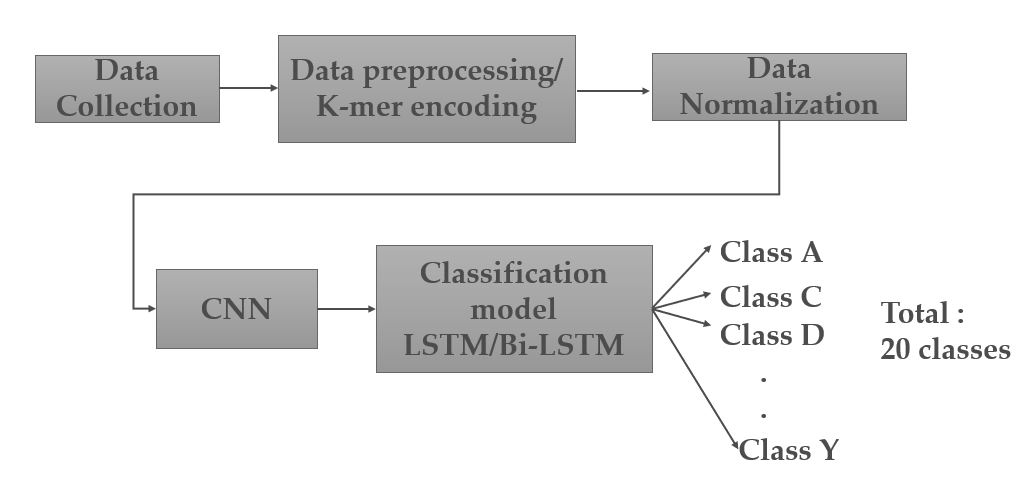
\includegraphics[width=8cm]{Model_Diagram.JPG}
      \caption{Model diagram for multi-classification of sequence data}
    \end{figure}

    \subsubsection{CNN}
    CNN is a powerful deep learning technique for feature extraction.
    CNN is often used on 2-dimensional and 3-dimensional datasets, e.g. image or video datasets.
    We use a 1-dimensional convolutional layer that convolves the kmers to extract any meaningful
    features. The convolutional layer has 128 filters with a kernel size of 3, so minimally the kmer-length cannot be
    smaller than 3. The feature maps from this layer forms as input to the LSTM or Bi-LSTM layer.

    \subsubsection{LSTM}
    Characteristic of the LSTM architecture is a set of chained together cells called "memory blocks". The number
    of memory blocks in the chain equals the length of the timesteps in our target dataset (Fig 2).
    Each memory cell has three gating units (forget, input and output gates) which
    conditionally regulate how information flows into and out of the memory block (Fig 3). Intuitively,
    the "forget" gate can be viewed as a step where irrelevant information from the hidden state
    is first "forgotten" before being passed to the input gate, which constructs the new cell state.
    Before that cell state can output its value to the next memory cell, it is filtered again through
    an output gate that decides what values to keep internal to the memory cell (i.e. the hidden state)
    and what to output to the next memory cell or final output layer.
    The LSTM layer is helpful, therefore, for learning the important sequence dependencies for performing
    sequence predictions.

    \subsubsection{Bidirectional LSTM}
        Bidirectional LSTM is a modification of the LSTM architecture that permits the model to learn both the
        forward and reverse dependencies. The way it acheives this is to have two LSTM layers, one consuming
        the timesteps in the forward direction and the other consuming the timesteps in the reverse direction.
        The two layers then merge their results to produce the final output.

    \begin{figure}[h]
      \centering
      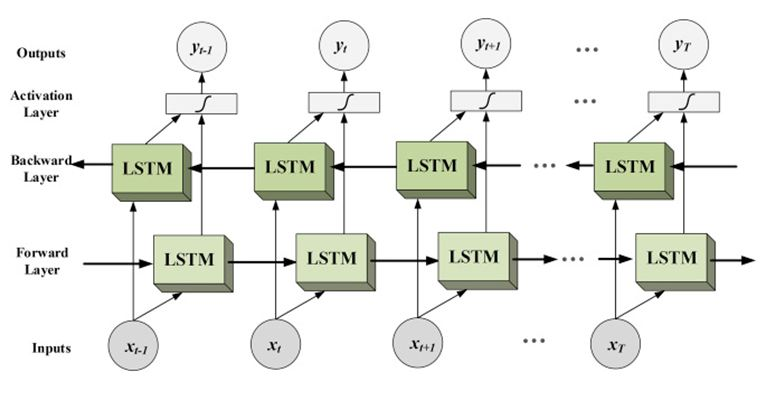
\includegraphics[width=8cm]{bidirectional-lstm.jpeg}
      \caption{Bidirectional LSTM Architecture}
    \end{figure}

    \begin{figure}[h]
    \centering
    \tikzstyle{place}=[rectangle,draw, thick, minimum width=30, minimum height=10]
    \begin{tikzpicture}
        \node at (0,0) [place] (first) {Memory Cell};
        \node at (3,0) [place] (second) {Memory Cell};
        \node at (6,0) [place] (third) {Memory Cell};
        % \draw [->] (0,0) -- (first.west);
        \draw [->] (first.east) -- (second.west);
        \draw [->] (second.east) -- (third.west);
        % \draw [->] (third.east) -- (10,0);
        \draw[decoration={brace,mirror,raise=10pt},decorate](first.south west) -- node[below=16pt] {Number of cells = number of time steps} (third.south east);
    \end{tikzpicture}
    \caption{Illustration of recurrently chained memory cells}
    \end{figure}

    \begin{figure}[h]
      \centering
      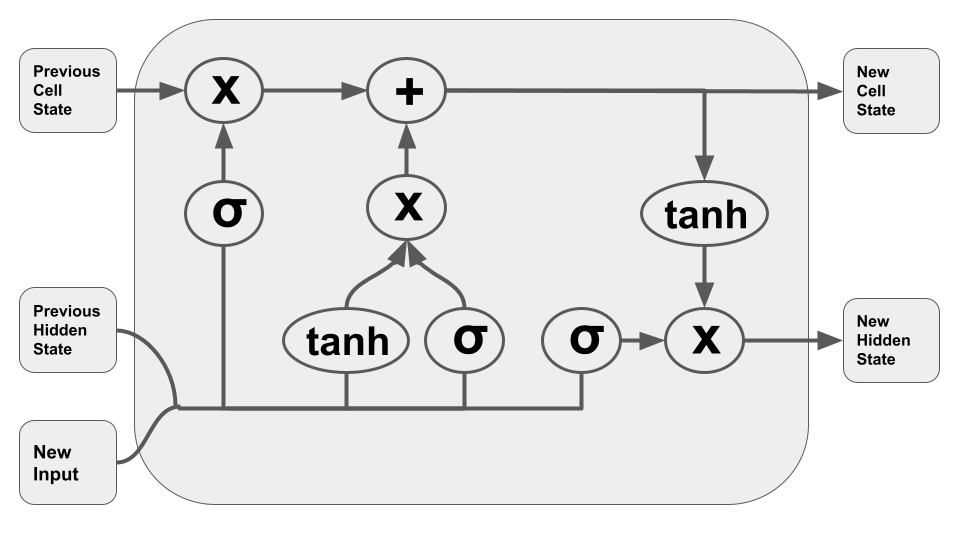
\includegraphics[width=8cm]{jordan_lstm_architecture.png}
      \caption{LSTM architecture inside a memory cell}
    \end{figure}

    \section{Model Architectures}

%   Model architecture: CNN / LSTM. Create diagram showing overall architecture. Discuss hyperparameters of model.

  \subsection{CNN}
  \subsection{LSTM}
  \subsection{LSTM-CNN}
  \subsection{BiLSTM-CNN}

\section{Experimental Results}
  Experimental results: Implementation process, tuning hyperparameters,
  show predictions in amino acid gaps
  (deploy the model and show its accuracy on a particular instance)
  \subsection{Tuning hyperparameters}
  \subsection{Accuracy/loss/confusion matrix/whatever}
  \subsection{Predictions on De Novo Sequence}

\section{Conclusion}
  Conclusion: Summarize project

\bibliographystyle{IEEEtran}
\bibliography{main}

% \begin{thebibliography}{10}

% \bibitem{cnn-hybrid}
%   H.~Gunasekaran, K.~Ramalakshmi, A.~Rex~Macedo~Arokiaraj, S.~Deepa~Kanmani, C.~Venkatesan, and C.~Suresh~Gnana~Dhas.
%   "Analysis of DNA Sequence Classification Using CNN and Hybrid Models."
%   \emph{Computational and mathematical methods in medicine}, 2021.
% \bibitem{IEEEhowto:kopka}
%   S.~Shadab,~M.~T.~Alam~Khan,~N.~A.~Neezi,~S.~Adilina,~and~S.~Shatabda,
%   “DeepDBP: deep neural networks for identification of DNA-binding proteins,”
%   \emph{Informatics in Medicine Unlocked}, vol. 19, article 100318, 2020.
% \bibitem{IEEEhowto:kopka}
%   M~.Pop and S~Salzberg. "Bioinformatics challenges of new sequencing technology."
%   \emph{Trends Genet}. vol. 24, no. 3, 142-149. 2008, doi: 10.1016/j.tig.2007.12.006.
% \bibitem{IEEEhowto:kopka}
%   S.~C.~Pakhrin,~B.~Shrestha,~B.~Adhikari,~and~D.~B.~Kc,
%   "Deep learning-based advances in protein structure prediction,"
%   \emph{Int. J. Mol. Sci.}, vol. 22, no. 11, 2021, doi: 10.3390/ijms22115553.
% \bibitem{IEEEhowto:kopka}
%   A.~Tasdelen and B.~Sen. "A hybrid CNN-LSTM model for pre-miRNA classification."
%   \emph{Scientific reports}, vol. 11, no. 1, 1-9. 2021.
% \bibitem{IEEEhowto:kopka}
%   J.~Chinju, O.~Matthew,~and~J.~Sahoo. "CNN-LSTM based classification of polo like kinase family of Proteins: An emerging cancer drug target."
%   \emph{Materials Today: Proceedings}, 2022.
% \bibitem{IEEEhowto:kopka}
%   S.~K.~Sønderby~and~O.~Winther, "Protein Secondary Structure Prediction with Long Short Term Memory Networks," 2014,
%   [Online]. Available: http://arxiv.org/abs/1412.7828.
% \bibitem{IEEEhowto:kopka}
%   N.~G.~Nguyen,~V.~A.~Tran,~D.~L.~Ngo et al., “DNA sequence classification by convolutional neural network,” \emph{Journal of Bio-
%   medical Science and Engineering}, vol. 9, no. 5, pp. 280–286, 2016.
% \bibitem{IEEEhowto:kopka}
%   D.~T.~Do~and~N.~Q.~K.~Le, “Using extreme gradient boosting to identify origin of replication in Saccharomyces cerevisiae via
%   hybrid features,” \emph{Genomics}, vol. 112, no. 3, pp. 2445–2451,2020
% \bibitem{IEEEhowto:kopka}
%   X.~Zhang,~B.~Beinke,~B.~Al~Kindhi,~and~M.~Wiering, “Comparing machine learning algorithms with or without feature extraction for DNA classification"
%   2020, http://arxiv.org/abs/2011.00485

% \end{thebibliography}
\end{document}
